\section{Conjectures}
% Here you can retake the examples of protocols in chapter 1. After explaining Maurer postulate, show that they don't violate Maurer because of reasons.
			\begin{quotation}
			Bound entanglement is a kind of correlation between Alice and Bob inaccessible to Eve but nevertheless of no use for generating a secret (quantum) key.\\
			Unfortunately the existence of such bound information, which would contradict the mentioned conjecture\footnotemark on the classical side of the picture, could not be proven so far.
		\end{quotation}
		
		\footnotetext{Shannon: Information theoretical security can be achieved only by parties sharing an unconditionally secret key initially. Maurer: this key can also not be generated from scratch. Maurer+Wolf: \emph{Intrinsic information} between $A$ and $B$ given $E$ == \emph{secret key rate}(how much key can Alice and Bob generate from that $P_{ABE}$).}
		
	%\lipsum[1]
	\section{State of research}
		\begin{figure}[h]
			\centering
			% scheme representing the bounds
% expresed in paper Renner+Wolf 2003
% on the quantities intrinsic information,
% secret key rate and information of formaion

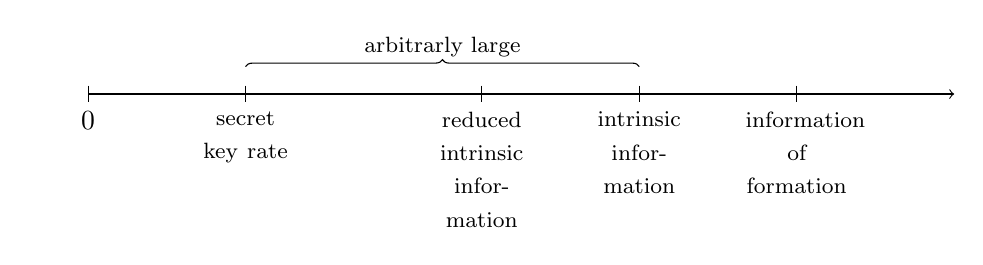
\begin{tikzpicture}
%	\tikzstyle{lineLabel}=[text width=10mm,align=center, below]
%	\draw[->] (0,0) -- (11,0);
%	\draw (0,.5) -- (0,-.5);
%	\draw (2,.5) -- (2,-.5);
%	\draw[dashed] (5,.5) -- (5,-.5);
%	\draw (7,.5) -- (7,-.5);
%	\draw (9,.5) -- (9,-.5);
%	
%	\node (zero) at (0,-.7) {$0$};
%	\node[lineLabel] (iof) at (9,-.7) {\footnotesize Information of formation};
%	\node[lineLabel] (inf) at (7,-.7) {\footnotesize Intrinsic Information};
%	\node[lineLabel] (rinf) at (5,-.7) {\footnotesize Reduced Intrinsic Information};
%	\node[lineLabel] (skr) at (2,-.7) {\footnotesize secret key rate};

\tikzset{
    position label/.style={
       below = 3pt,
       align=center,
%       text height = 1.5ex,
%       text depth = 1ex,
       text width=13mm
    },
   brace/.style={
     decoration={brace},
     decoration={raise=3ex},
     decorate
   },
   blabel/.style={
		above = 13pt,
		align=center,
		pos=0.5   
   }
}

% draw horizontal line
\draw[->] (0,0) -- (11,0);

%draw vertical lines
\foreach \x in {0,2,5,7,9}
   \draw (\x cm,3pt) -- (\x cm,-3pt);

%labels
\node [position label] (Start) at (0,0) {$0$};
\node [position label] (skr) at (2,0) {\footnotesize secret key rate};
\node [position label] (rinf) at (5,0) {\footnotesize reduced intrinsic information};
\node [position label] (inf) at (7,0) {\footnotesize intrinsic information};
\node [position label] (iof) at (9,0) {\footnotesize information of formation};

\draw [brace] (skr.north) -- node [blabel] {\footnotesize arbitrarly large} (inf.north);

\end{tikzpicture}
			\caption{Bounds on the quantities as stated in Wolf + Renner 2003 proceeding}
		\end{figure}
	%\lipsum[1]
	\section{My considerations}
	%\lipsum[1]
